\documentclass[10pt,twocolumn]{article}

\usepackage[margin=0.72in]{geometry}
\usepackage{amsmath,amssymb}
\usepackage{booktabs}
\usepackage{array}
\usepackage{url}
\usepackage{graphicx}
\usepackage{float}
\usepackage{tikz}
\usetikzlibrary{arrows.meta,positioning}
\usepackage{hyperref}

\title{\vspace{-0.4in}H-Infinity Lateral Steering Control Design for a Linear Bicycle Vehicle Model}
\author{Yupeng Zhou}
\date{}

\begin{document}
\maketitle

\begin{abstract}
This report presents the derivation, formulation, and simulation evaluation of an
$H_\infty$ lateral steering controller for a constant-speed ground vehicle. The
plant is modeled as a linear bicycle model with lateral position, yaw angle,
lateral velocity, and yaw rate states. A side-wind-speed input is added by
linearizing the lateral aerodynamic force and applying it at the vehicle center
of gravity. The controller is synthesized in MATLAB using named-signal block
interconnection and \texttt{hinfsyn}. The weighted generalized plant includes
lateral tracking-error performance, steering command shaping, side-wind
disturbance shaping, and optional measurement-noise channels. The final
closed-loop analysis is performed with an unweighted augmented plant and
linear fractional transformation (LFT), so the reported responses correspond to
the physical lateral plant rather than the weighted synthesis model.
\end{abstract}

\section{Introduction}

Automatic steering can be formulated as a robust lateral tracking problem in
which the steering input must regulate vehicle lateral position and heading in
the presence of disturbances and modeling uncertainty. Rafaila and Livint
studied a related $H_\infty$ automatic steering problem for a vehicle moving at
constant speed, using loop-shaping ideas and closed-loop simulation to evaluate
steering performance \cite{rafaila2016}. This project follows the same
constant-speed steering setting, but implements the full MATLAB design workflow
for the current AlpaSim-style lateral model.

The main contributions of this project are:
\begin{itemize}
    \item derivation of a lateral-only state-space bicycle model using the
    rear/rig lateral position as the tracked position;
    \item inclusion of a signed side-wind-speed disturbance by local
    aerodynamic-force linearization;
    \item construction of an $H_\infty$ generalized plant using MATLAB named
    signals and \texttt{connect};
    \item construction of clean and noisy closed-loop analysis models using
    \texttt{lft} around the original unweighted plant;
    \item implementation of reusable time-domain tracking simulations for
    trajectory tracking and wind-disturbance rejection.
\end{itemize}

\section{Vehicle Lateral Dynamics}

\subsection{Modeling Assumptions}

The model is a lateral-only linear bicycle model. The longitudinal speed is
held constant at
\begin{equation}
    v_x = 10~\mathrm{m/s}.
\end{equation}
The small-angle and small-slip assumptions are used, tire forces are assumed
linear in slip angle, and longitudinal, roll, tire-saturation, and hard actuator
saturation effects are neglected. The steering command is applied directly as
the front steering angle. Side wind is modeled as a lateral force acting at the
center of gravity (CG), so it has no direct yaw moment.

The lateral state vector is
\begin{equation}
    x =
    \begin{bmatrix}
        y_{\mathrm{rig}} & \psi & v_y & r
    \end{bmatrix}^{T},
\end{equation}
where $y_{\mathrm{rig}}$ is the lateral position of the rear/rig reference
point, $\psi$ is yaw angle, $v_y$ is lateral velocity at the CG, and $r$ is yaw
rate. The plant input vector is
\begin{equation}
    u =
    \begin{bmatrix}
        \delta & v_w
    \end{bmatrix}^{T},
\end{equation}
where $\delta$ is steering command and $v_w$ is signed side-wind speed.

\subsection{Linear Tire Forces}

Let $l_f$ and $l_r$ be the distances from the CG to the front and rear
reference points, and let $C_{af}$ and $C_{ar}$ be the front and rear cornering
stiffnesses. The linearized front and rear lateral tire forces are
\begin{align}
    F_{yf} &=
    2 C_{af}
    \left(
        \delta - \frac{v_y + l_f r}{v_x}
    \right), \label{eq:front_force}\\
    F_{yr} &=
    2 C_{ar}
    \left(
        -\frac{v_y - l_r r}{v_x}
    \right). \label{eq:rear_force}
\end{align}

The lateral and yaw equations of motion are
\begin{align}
    m\left(\dot{v}_y + v_x r\right) &=
    F_{yf} + F_{yr} + F_w, \label{eq:lateral_eom}\\
    I_z \dot{r} &=
    l_f F_{yf} - l_r F_{yr}. \label{eq:yaw_eom}
\end{align}

\subsection{Side-Wind Linearization}

The nonlinear aerodynamic side force is modeled as
\begin{equation}
    F_w =
    \frac{1}{2}\rho C_y A_s |v_w|v_w ,
\end{equation}
where $\rho$ is air density, $C_y$ is the side-force coefficient, and $A_s$ is
the side projected area. Around a nonzero operating wind speed
$v_{w0}$, the local linearization is
\begin{equation}
    \Delta F_w
    \approx
    k_w \Delta v_w,
    \qquad
    k_w =
    \rho C_y A_s |v_{w0}|.
\end{equation}
Since the force is applied at the CG, the direct yaw moment from wind is zero.
Thus the wind input enters only through the lateral acceleration equation.

\subsection{State-Space Form}

The kinematics of the rear/rig reference point are
\begin{align}
    \dot{y}_{\mathrm{rig}} &=
    v_x \psi + v_y - l_r r, \label{eq:y_kinematics}\\
    \dot{\psi} &= r. \label{eq:yaw_kinematics}
\end{align}

Combining \eqref{eq:front_force}--\eqref{eq:yaw_kinematics} gives
\begin{equation}
    \dot{x} = A x + B u,
    \qquad
    y = C x + D u ,
\end{equation}
where
\begin{equation}
    A =
    \begin{bmatrix}
        0 & v_x & 1 & -l_r \\
        0 & 0 & 0 & 1 \\
        0 & 0 & a_{00} & a_{01} \\
        0 & 0 & a_{10} & a_{11}
    \end{bmatrix},
\end{equation}
\begin{equation}
    B =
    \begin{bmatrix}
        0 & 0 \\
        0 & 0 \\
        b_{00} & k_w/m \\
        b_{10} & 0
    \end{bmatrix},
\end{equation}
and
\begin{align}
    a_{00} &=
    -\frac{2(C_{af}+C_{ar})}{m v_x},\\
    a_{01} &=
    -v_x
    -\frac{2(l_f C_{af}-l_r C_{ar})}{m v_x},\\
    a_{10} &=
    -\frac{2(l_f C_{af}-l_r C_{ar})}{I_z v_x},\\
    a_{11} &=
    -\frac{2(l_f^2 C_{af}+l_r^2 C_{ar})}{I_z v_x},\\
    b_{00} &= \frac{2C_{af}}{m},\\
    b_{10} &= \frac{2l_f C_{af}}{I_z}.
\end{align}
The current implementation uses $C=I_4$, so all four states are available as
analysis outputs.

\section{Control Problem Formulation}

The objective is to synthesize a steering controller that reduces lateral
tracking error while rejecting side-wind disturbances. The measured lateral
tracking error used by the current controller is
\begin{equation}
    e_y = r_y - y_{\mathrm{rig},ns},
\end{equation}
where $r_y$ is the lateral reference and $y_{\mathrm{rig},ns}$ is the possibly
noisy measured lateral position.

The generalized plant input vector used for synthesis is
\begin{equation}
    w =
    \begin{bmatrix}
        r_y & r_\psi & n_y & n_\psi & d_w
    \end{bmatrix}^{T},
    \qquad
    u_c = \delta_{\mathrm{in}},
\end{equation}
where $d_w$ is the shaped side-wind input and $u_c$ is the controller output.
The active performance output is
\begin{equation}
    z = W_{a_y}(s)e_y .
\end{equation}
The controller measurement is
\begin{equation}
    y_c = e_y .
\end{equation}

The MATLAB command
\begin{equation}
    [K_1,S_{\mathrm{cl}},\gamma] =
    \texttt{hinfsyn}(P,n_{\mathrm{meas}},n_{\mathrm{cont}})
\end{equation}
solves the standard $H_\infty$ problem
\begin{equation}
    \min_{K_1} \left\| T_{zw}(s) \right\|_\infty ,
\end{equation}
where $T_{zw}$ is the closed-loop transfer matrix from exogenous inputs $w$ to
weighted performance outputs $z$. In the current code,
\begin{equation}
    n_{\mathrm{meas}} = 1,
    \qquad
    n_{\mathrm{cont}} = 1.
\end{equation}
Therefore the final generalized-plant output is treated as the controller
measurement and the final generalized-plant input is treated as the controller
command.

\section{Block Interconnection}

\begin{figure*}[t]
\centering
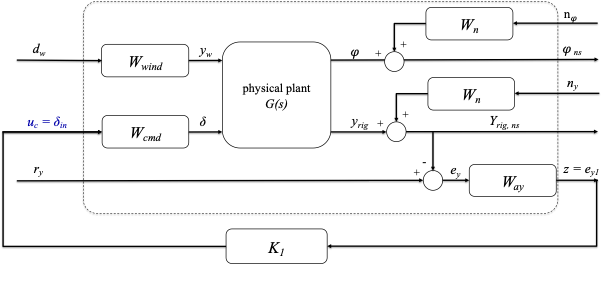
\includegraphics[width=0.98\textwidth]{../img/block.png}
\caption{Generalized-plant interconnection used for $H_\infty$ synthesis. The
dashed box is $P(s)$ and includes the physical plant, weighting filters, and
summing junctions. The controller $K_1$ is outside $P(s)$, receives the measured
tracking error $y_c=e_y$, and returns the normalized steering command
$u_c=\delta_{\mathrm{in}}$.}
\label{fig:block_interconnection}
\end{figure*}

\subsection{Synthesis Plant}

The synthesis plant, named \texttt{nominal\_op} in MATLAB, is built from:
\begin{itemize}
    \item \texttt{lateral\_sys}: original physical state-space plant;
    \item \texttt{Rpass}: reference pass-through block;
    \item \texttt{Wn}: measurement-noise scaling block;
    \item \texttt{Wa\_y}: lateral tracking-error performance weight;
    \item \texttt{Wa\_yaw}: yaw tracking weight, currently defined but not active;
    \item \texttt{W\_cmd}: steering command shaping block;
    \item \texttt{W\_wind}: side-wind disturbance shaping block.
\end{itemize}

The current synthesis output list is
\begin{equation}
    \left[
        e_{y1},\; e_y
    \right]^T,
\end{equation}
where $e_{y1}=W_{a_y}e_y$. Thus, only the lateral position error is currently
included in the $H_\infty$ performance objective. The yaw error is computed and
plotted for analysis, but $e_{\psi 1}$ is not presently included in the
synthesis output vector.

\subsection{Unweighted Closed-Loop Analysis Plant}

After synthesis, the controller $K_1$ maps
\begin{equation}
    e_y \mapsto \delta_{\mathrm{in}}.
\end{equation}
The physical plant expects the physical steering command $\delta$, so the
implemented controller used for closed-loop analysis is
\begin{equation}
    K_{\mathrm{plant}}(s) = W_{\mathrm{cmd}}(s)K_1(s).
\end{equation}

The clean analysis plant is named
\texttt{nominal\_augment\_lateral\_system}. It is built from the original
unweighted plant and error-summing blocks. The closed-loop model is obtained by
\begin{equation}
    \mathrm{CL}_1 =
    \mathcal{F}_{l}
    \left(
        \mathrm{nominal\_augment\_lateral\_system},
        K_{\mathrm{plant}}
    \right),
\end{equation}
where $\mathcal{F}_l(\cdot,\cdot)$ denotes the lower linear fractional
transformation. This model has physical external inputs
\begin{equation}
    \left[
        r_y,\; r_\psi,\; v_w
    \right]^T
\end{equation}
and analysis outputs
\begin{equation}
    \left[
        y_{\mathrm{rig}},\; \psi,\; v_y,\; r,\; e_y,\; e_\psi
    \right]^T .
\end{equation}
This separation is important because the tracking and disturbance weights are
used for synthesis, but they are not interpreted as physical vehicle dynamics
in the final analysis.

\section{Weighting Design}

\subsection{Lateral Tracking Weight}

The lateral tracking weight is
\begin{equation}
    W_{a_y}(s)
    =
    \frac{1}{e_{y,\max}}
    \frac{\omega_b}{s+\omega_b},
\end{equation}
where
\begin{equation}
    e_{y,\max}=0.18~\mathrm{m},
    \qquad
    \omega_b = 2\pi(0.5)~\mathrm{rad/s}.
\end{equation}
At low frequency,
\begin{equation}
    |W_{a_y}(0)| =
    \frac{1}{0.18}
    =
    5.56~\mathrm{m}^{-1}.
\end{equation}
Thus the design asks the controller to keep low-frequency lateral error below
approximately $0.18$ m. Above the selected bandwidth, the weight rolls off and
high-frequency tracking error is penalized less strongly.

\subsection{Yaw Tracking Weight}

The yaw tracking weight is defined as
\begin{equation}
    W_{a_\psi}(s)
    =
    \frac{1}{e_{\psi,\max}}
    \frac{\omega_b}{s+\omega_b},
    \qquad
    e_{\psi,\max}=0.3~\mathrm{rad}.
\end{equation}
However, this weight is not currently active in synthesis because the current
generalized-plant output vector does not include $W_{a_\psi}e_\psi$. If heading
tracking is a formal design requirement, the output vector should include both
weighted errors.

\subsection{Steering Command Weight}

The steering command shaping block is
\begin{equation}
    W_{\mathrm{cmd}}(s)
    =
    \frac{0.5}{(0.05/\pi)s+1}.
\end{equation}
This maps the normalized controller command to the physical steering command.
Its DC gain is $0.5$ rad and its pole is approximately $62.8$ rad/s. This block
shapes the steering path, but it is not a hard saturation model.

\subsection{Side-Wind Weight}

The side-wind disturbance weight is
\begin{equation}
    W_{\mathrm{wind}}(s)
    =
    \frac{4.9}{s+1}.
\end{equation}
The low-frequency gain represents a wind disturbance on the order of several
meters per second, while the pole at $1$ rad/s emphasizes slow and step-like
wind changes. If the expected operating scenario is a larger sudden gust, the
DC gain and pole of $W_{\mathrm{wind}}$ should be selected to match that
disturbance model.

\section{Simulation and Robustness Results}

Running the current MATLAB script gives the open-loop poles
\begin{equation}
    p =
    \left[
        0,\;0,\;-22.1741,\;-39.3899
    \right].
\end{equation}
The two poles at the origin come from the lateral-position and yaw-angle
integrators. The latest $H_\infty$ synthesis result is
\begin{equation}
    \gamma = 0.4641.
\end{equation}
Since $\gamma<1$, the active weighted lateral-error objective is feasible for
the shaped synthesis plant.

\begin{figure}[H]
\centering
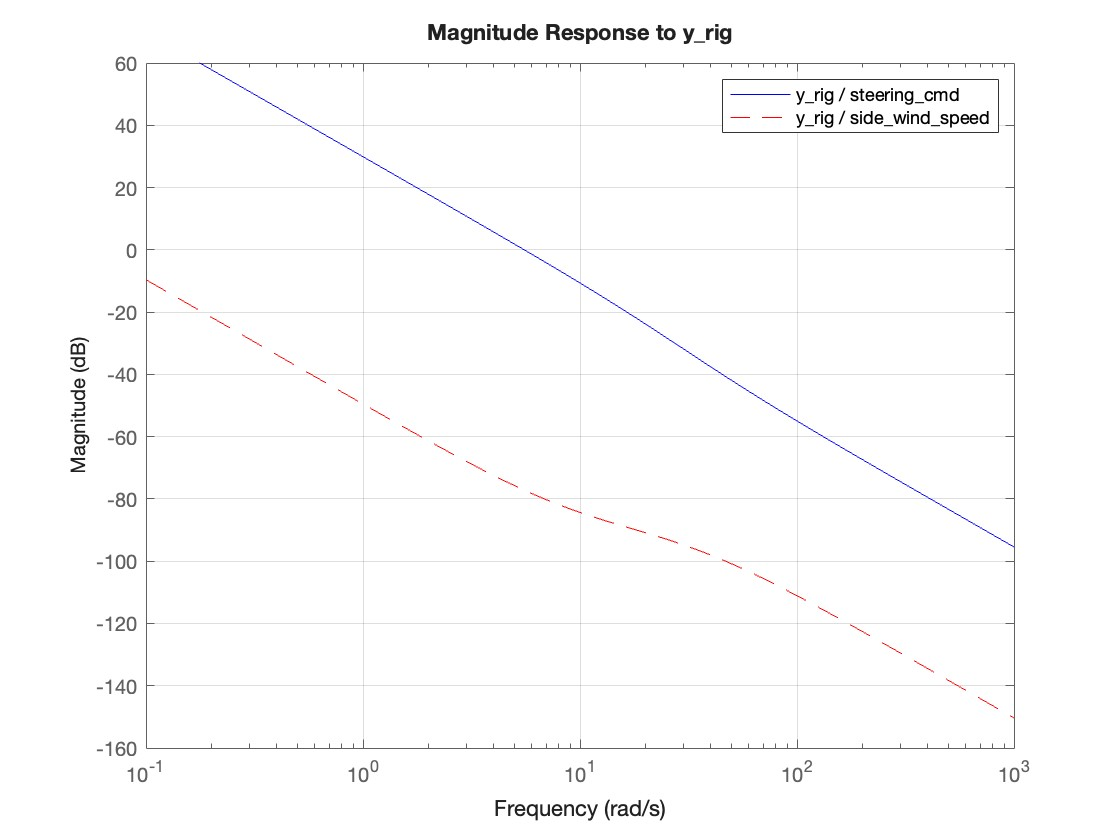
\includegraphics[width=0.9\columnwidth]{../img/1.jpg}\\[0.5em]
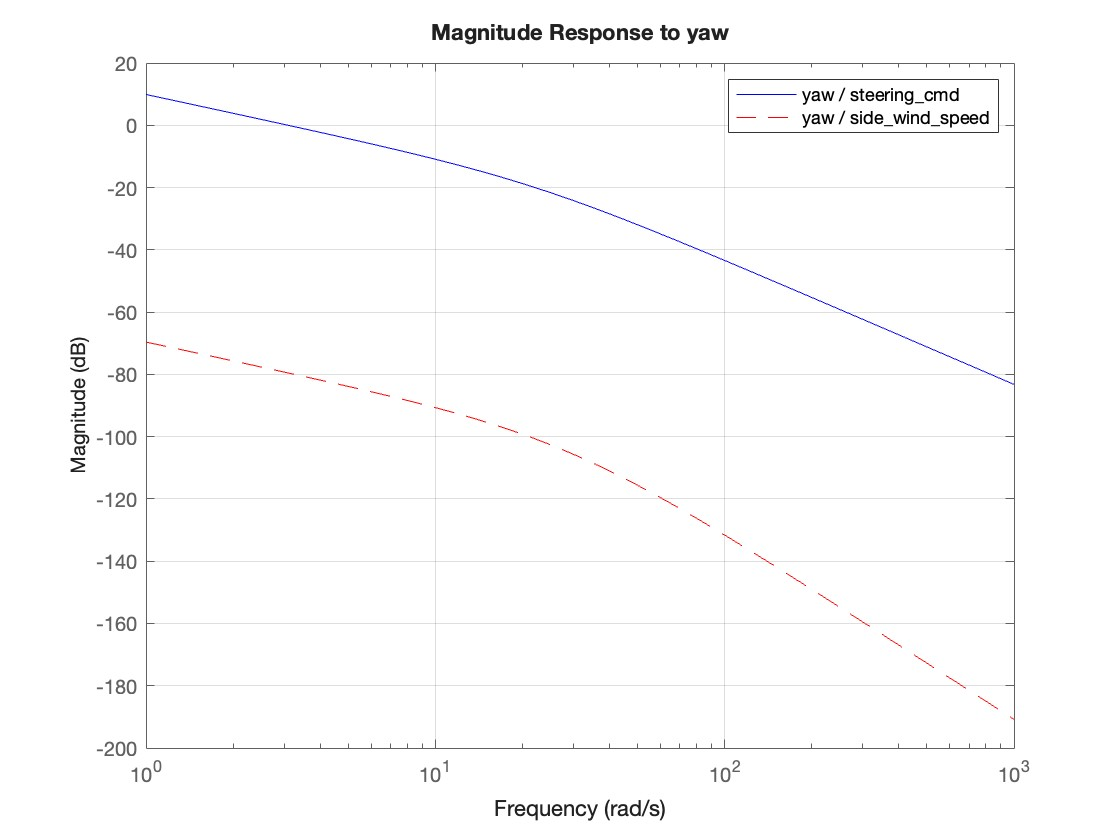
\includegraphics[width=0.9\columnwidth]{../img/2.jpg}
\caption{Open-loop plant magnitude responses from steering command and
side-wind speed to lateral position and yaw. Steering has much larger authority
than the side-wind channel, while the side-wind-to-yaw transfer is very small
because wind force is applied at the CG.}
\label{fig:open_loop_bode}
\end{figure}

\begin{figure}[H]
\centering
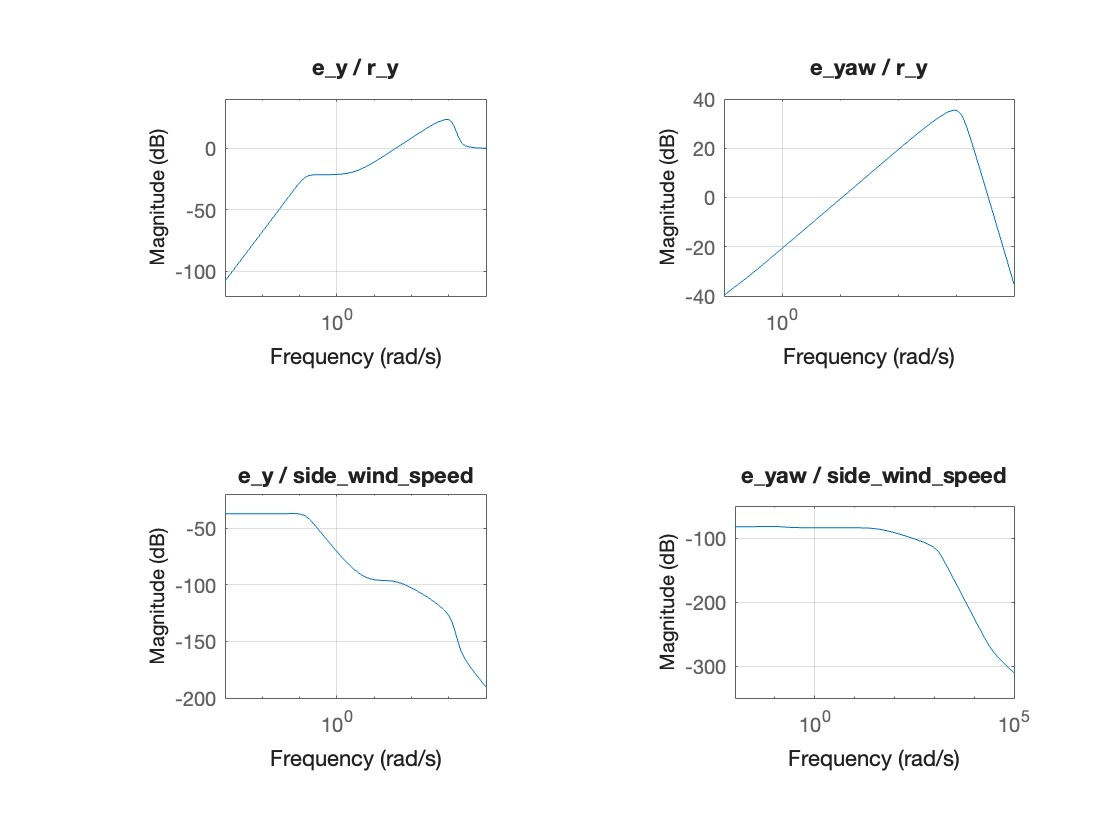
\includegraphics[width=0.9\columnwidth]{../img/3.jpg}\\[0.5em]
% 
\includegraphics[width=0.98\columnwidth]{4.jpg}
\caption{Nominal closed-loop tracking-error magnitude responses without and
with the measurement-noise channels. The two plots are visually identical here
because the current noise weights are set to zero in the MATLAB script.}
\label{fig:closed_loop_bode}
\end{figure}
\clearpage

\begin{table}[H]
\centering
\caption{Current time-domain simulation results}
\resizebox{\columnwidth}{!}{%
\begin{tabular}{lccc}
\toprule
Case & Reference & Wind & Peak $|e_y|$ \\
\midrule
No side wind & default S path, $\pm 2$ m & $0$ m/s & $0.264$ m \\
Wind step & $0$ m & $8$ m/s at $5$ s & $0.246$ m \\
\bottomrule
\end{tabular}
}
\label{tab:simulation_results}
\end{table}

The two cases in Table~\ref{tab:simulation_results} should not be compared as
a direct wind/no-wind performance pair because they use different references.
The no-wind case evaluates nominal trajectory tracking, while the wind-step
case isolates disturbance rejection with zero lateral reference. A fair
comparison should use the same reference trajectory and only change the
side-wind input.

\begin{figure}[H]
\centering
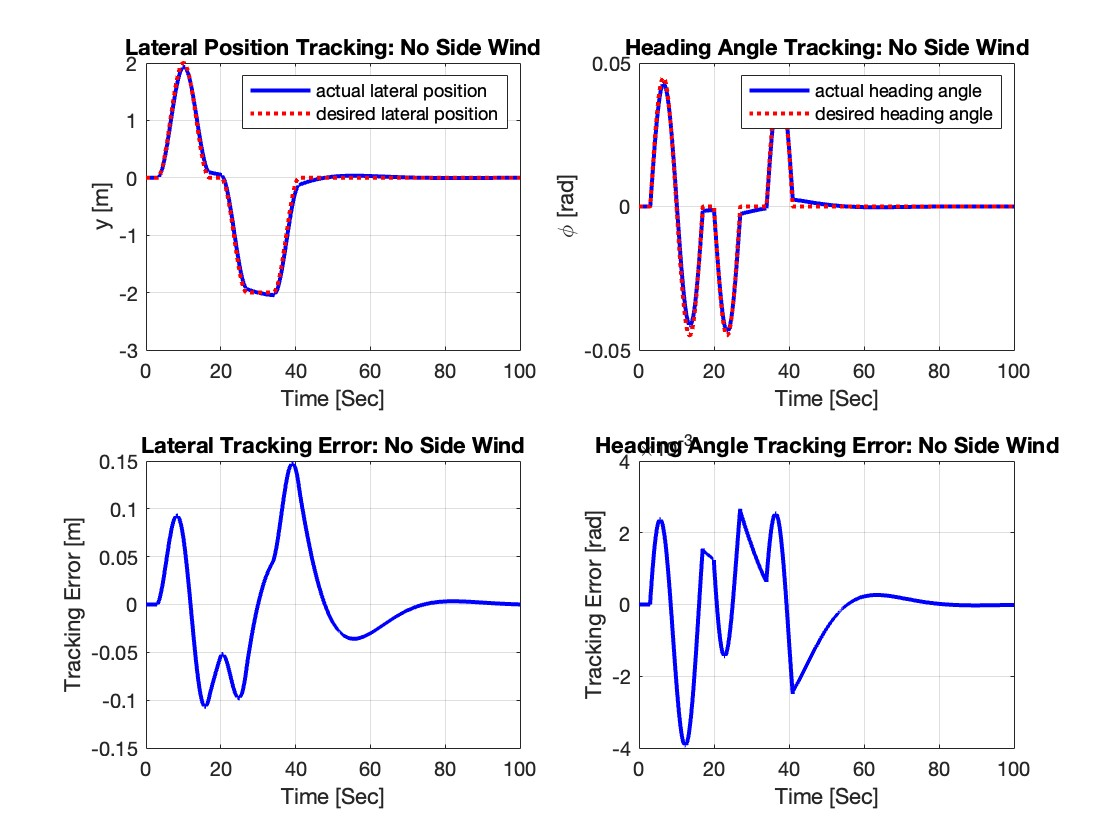
\includegraphics[width=0.98\columnwidth]{../img/5.jpg}\\[0.5em]
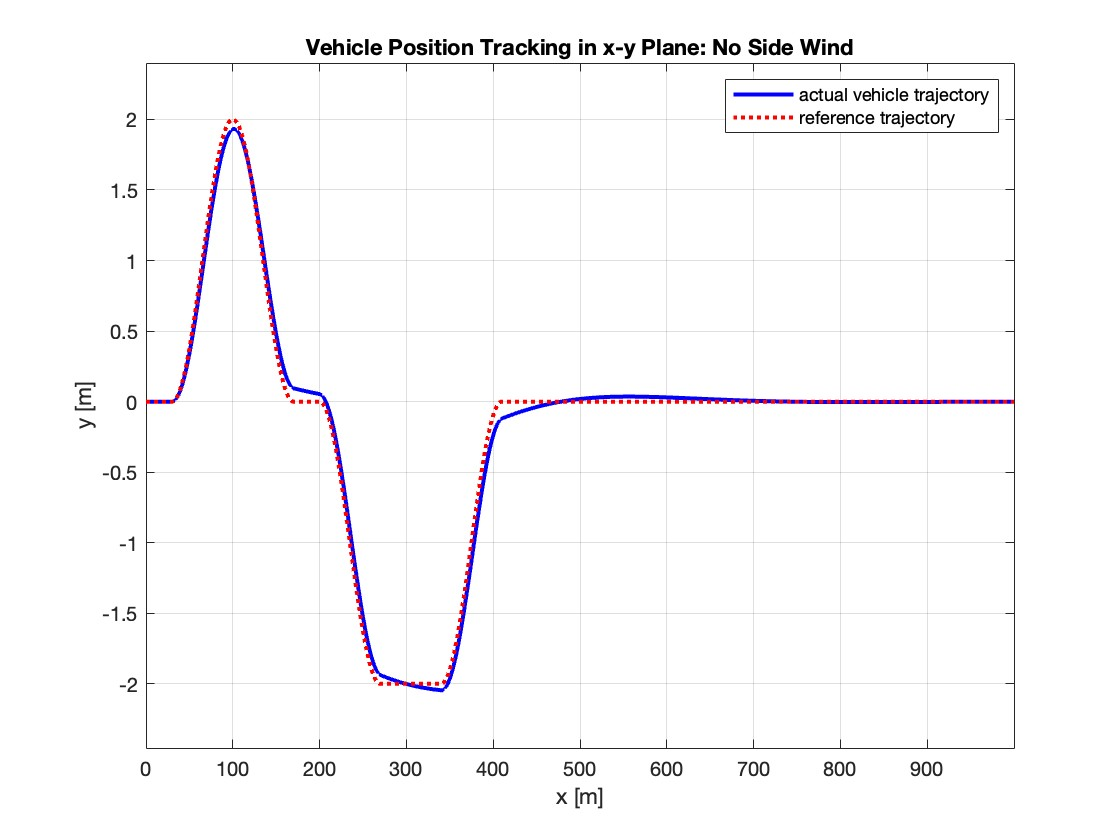
\includegraphics[width=0.98\columnwidth]{../img/6.jpg}
\caption{Nominal closed-loop tracking of the S-shaped lateral reference with no
side wind. The lateral position follows the $\pm 2$ m path with small transient
offset, and the reconstructed $x$-$y$ trajectory confirms that the physical
vehicle path follows the desired lane-change shape.}
\label{fig:nominal_tracking}
\end{figure}

\begin{figure}[H]
\centering
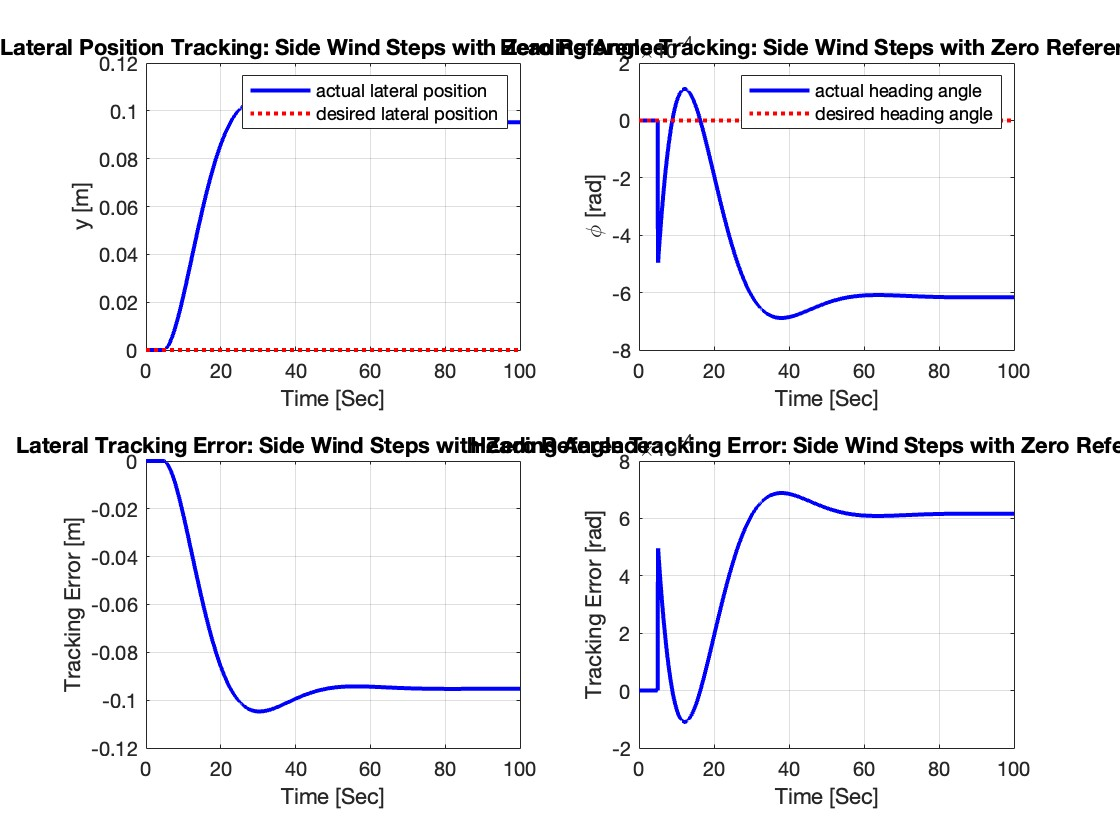
\includegraphics[width=0.98\columnwidth]{../img/7.jpg}\\[0.5em]
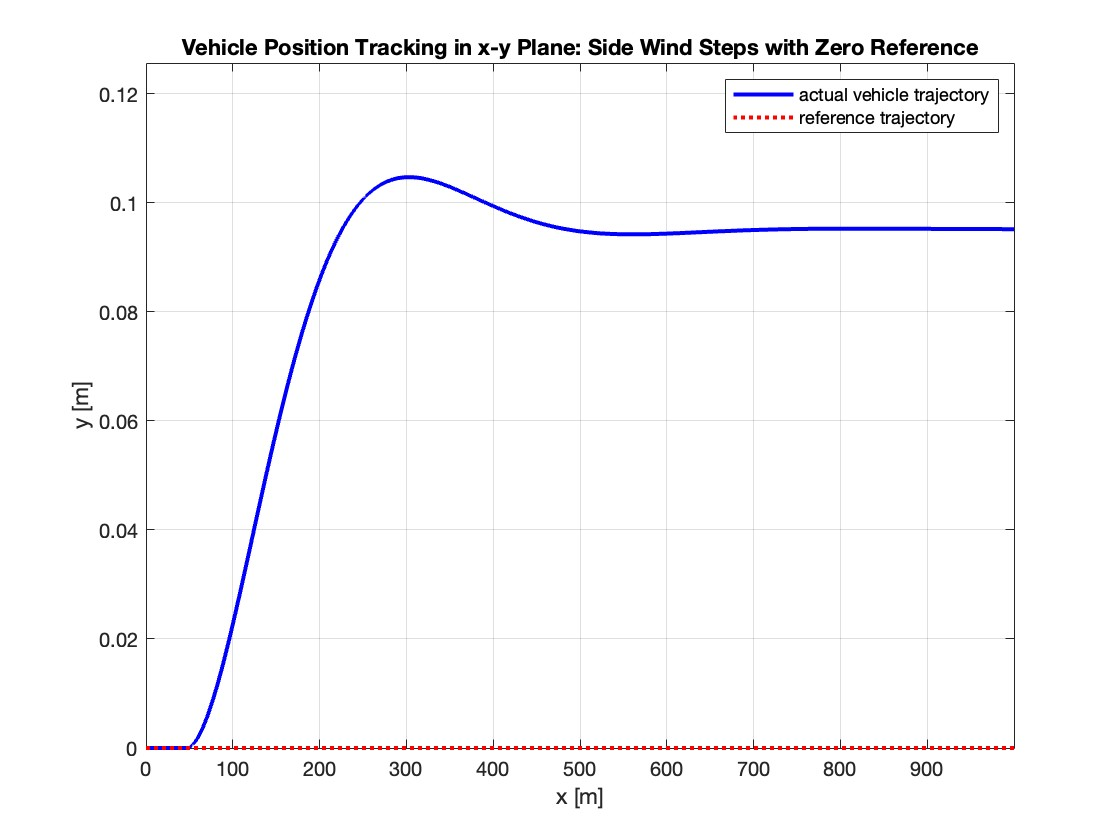
\includegraphics[width=0.98\columnwidth]{../img/8.jpg}
\caption{Nominal closed-loop response to an 8 m/s side-wind step with zero
lateral reference. The controller limits the lateral displacement to roughly
0.1 m, but the yaw response is large because yaw tracking is not part of the
active synthesis objective.}
\label{fig:wind_tracking}
\end{figure}

\subsection{Parametric Uncertainty}

Robustness is evaluated by replacing the nominal mass and tire cornering
stiffnesses with uncertain real parameters. The uncertainty set used for the
reported MATLAB run is
\begin{equation}
    m \in [-5\%,+15\%],
    \qquad
    C_{af}, C_{ar} \in [-10\%,0\%],
\end{equation}
relative to their nominal values. The nominal $H_\infty$ controller is then
closed around the uncertain physical plant and tested using robust stability,
robust performance, and sampled closed-loop simulations.

\begin{table}[H]
\centering
\caption{Robustness and $\mu$-synthesis command results}
\resizebox{\columnwidth}{!}{%
\begin{tabular}{lc}
\toprule
Quantity & Result \\
\midrule
$H_\infty$ synthesis $\gamma$ & 0.4641 \\
Robust stability margin, nominal controller & $[0.2129,\;0.2133]$ \\
Robust performance margin at $\gamma=1$ & $[0.1320,\;0.1323]$ \\
Best $\mu$-synthesis robust performance & 1.03 \\
Final \texttt{musyn} robust performance & 1.0258 \\
$\mu$ controller nominal closed-loop stable & true \\
\bottomrule
\end{tabular}
}
\label{tab:robust_results}
\end{table}

The robust stability margin is below one, so the nominal $H_\infty$ controller
is not certified to stabilize the full uncertainty set. A margin of about
0.213 means the closed loop can tolerate only about 21\% of the modeled
uncertainty size before worst-case instability may occur. The robust performance
margin is even smaller, which means the weighted tracking-performance target is
lost before the worst-case stability boundary is reached.

\begin{figure}[H]
\centering
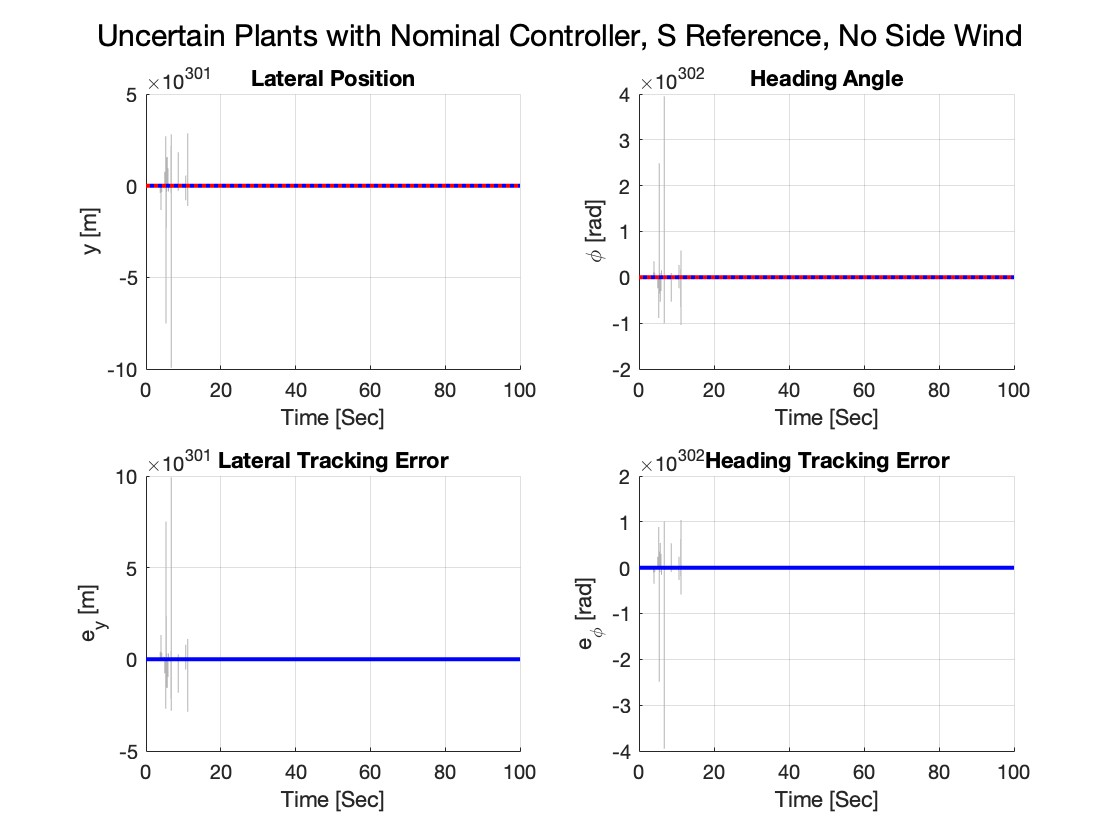
\includegraphics[width=0.98\columnwidth]{../img/9.jpg}
\caption{Sampled uncertain plants with the nominal $H_\infty$ controller for
the S-shaped reference and zero side wind. Several sampled responses diverge,
which is consistent with the robust stability margin being far below one.}
\label{fig:uncertain_samples}
\end{figure}

\section{\texorpdfstring{$\mu$-Synthesis Controller Design}{Mu-Synthesis Controller Design}}

Because the nominal $H_\infty$ controller is not certified for the full
uncertainty set, a structured robust controller is also designed using MATLAB
\texttt{musyn}. The same uncertain generalized plant, input/output ordering,
single controller measurement $e_y$, and single controller command
$\delta_{\mathrm{in}}$ are used. The implemented physical controller is
\begin{equation}
    K_{\mu,\mathrm{plant}}(s) =
    W_{\mathrm{cmd}}(s)K_{\mu}(s),
\end{equation}
so the controller output is converted to the physical steering command before
closing the loop around the vehicle plant.

\texttt{musyn} applies D-K iteration. In each iteration, the K step synthesizes
a controller for the scaled problem, then the D step fits frequency-dependent
scalings that upper-bound the structured singular value. The command output in
Table~\ref{tab:dk_iteration} shows that the peak $\mu$ value decreases from
6.358 in the first iteration to 1.026 by the ninth iteration.

\begin{table}[H]
\centering
\caption{D-K iteration summary from \texttt{musyn}}
\resizebox{\columnwidth}{!}{%
\begin{tabular}{ccccc}
\toprule
Iter. & K step & Peak $\mu$ & D fit & D order \\
\midrule
1 & $2.695{\times}10^{6}$ & 6.358 & 6.423 & 46 \\
2 & 1.638 & 1.504 & 1.514 & 20 \\
3 & 1.205 & 1.205 & 1.212 & 26 \\
4 & 1.097 & 1.097 & 1.100 & 28 \\
5 & 1.063 & 1.063 & 1.065 & 30 \\
6 & 1.050 & 1.049 & 1.051 & 32 \\
7 & 1.038 & 1.036 & 1.038 & 32 \\
8 & 1.034 & 1.033 & 1.037 & 32 \\
9 & 1.026 & 1.026 & 1.026 & 32 \\
\bottomrule
\end{tabular}
}
\label{tab:dk_iteration}
\end{table}

The best achieved robust performance reported by \texttt{musyn} is about
1.03, and the final returned value is 1.0258. This is a substantial improvement
over the nominal $H_\infty$ robust-performance margin, but the value is still
slightly above one. Therefore the $\mu$-synthesis controller improves the
robust design, but it still does not fully certify robust performance over the
complete modeled uncertainty set.

\begin{figure}[H]
\centering
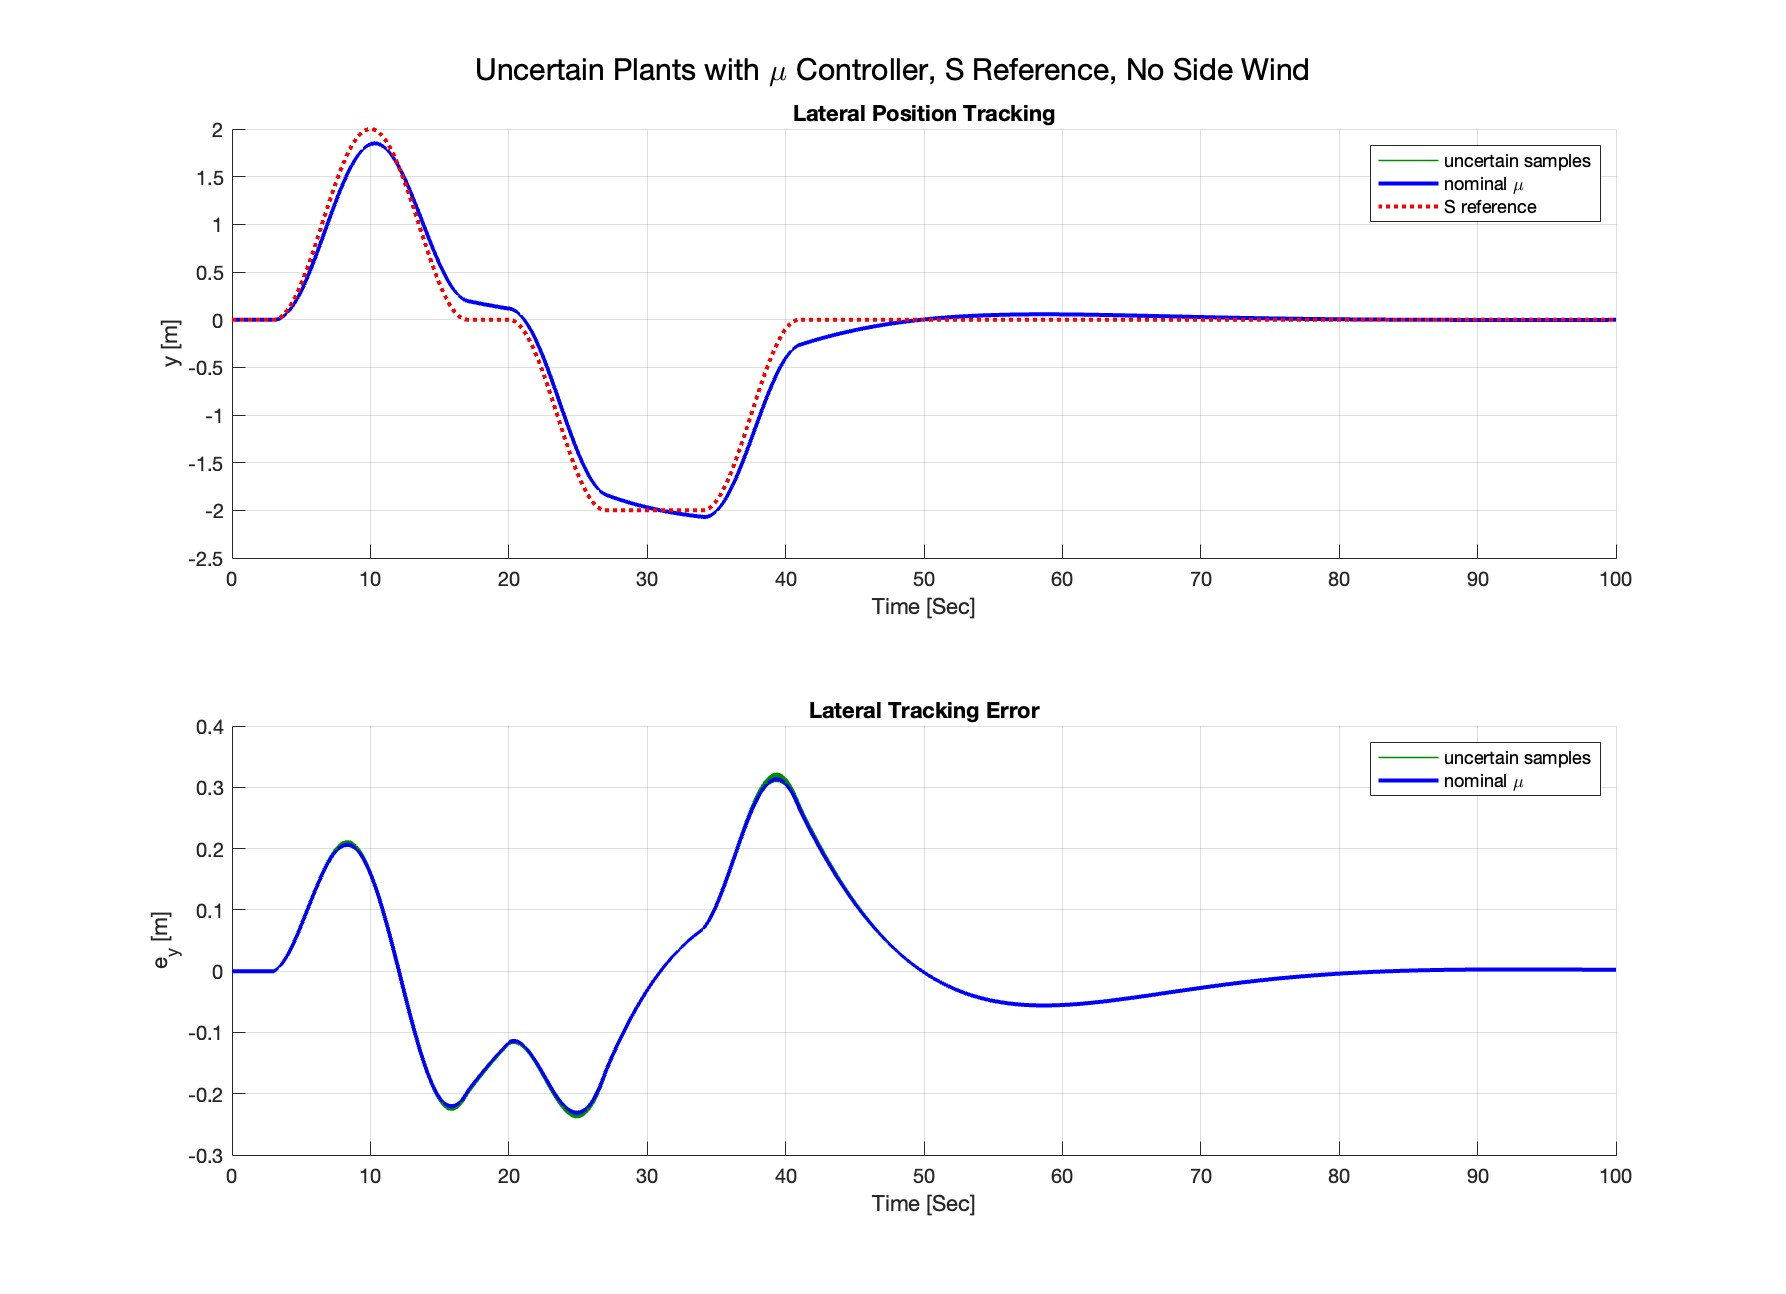
\includegraphics[width=0.98\columnwidth]{../img/12.jpg}
\caption{Sampled uncertain plants with the $\mu$-synthesis controller for the
S-shaped reference and zero side wind. The green responses show the sampled
uncertain closed-loop plants, the blue response is the nominal $\mu$ controller
response, and the red dotted curve is the reference trajectory.}
\label{fig:mu_uncertain_samples}
\end{figure}

\section{Discussion}

The current design achieves $\gamma<1$ for the active nominal lateral-position
tracking objective, but the robust analysis shows that nominal $H_\infty$
performance is not enough to guarantee behavior over the modeled mass and tire
uncertainty. The sampled uncertain responses in Fig.~\ref{fig:uncertain_samples}
show why the robust margin matters: a controller that tracks well on the nominal
plant can still become unstable for admissible uncertain plants. The
$\mu$-synthesis sampled responses in Fig.~\ref{fig:mu_uncertain_samples} show
that the structured robust design moves the closed-loop behavior closer to
robust feasibility, but the achieved robust performance is still above one.

Several limitations remain. First, the yaw performance weight is defined but
not active in the $H_\infty$ or $\mu$-synthesis performance output. Second, the
steering command block shapes steering authority but does not enforce hard angle
or rate limits. Third, the wind model is a local linearization around a selected
operating wind speed, so very small or very large wind speeds may differ from
the nonlinear aerodynamic force law. Finally, the weight $W_{a_y}$ specifies an
absolute error target in meters, not a percentage error target. If percentage
tracking error is required, the error channel should be normalized by a chosen
reference scale.

\section{Conclusion}

This project constructs a complete MATLAB $H_\infty$ lateral steering design
workflow for a constant-speed linear bicycle model. The final code separates
the physical plant, the weighted synthesis plant, and the unweighted LFT
analysis plant. This makes the design easier to interpret: the weights guide
controller synthesis, while the final closed-loop simulations evaluate the
controller on the original vehicle dynamics. The current controller satisfies
the active nominal weighted lateral-error objective, but robust analysis shows
that the full modeled uncertainty range is not certified. The $\mu$-synthesis
controller improves the robust objective but still gives a robust-performance
value slightly above one. Future work should activate yaw tracking in the
synthesis objective, verify steering saturation and rate limits, and either
relax the tracking weight or reduce the uncertainty set to obtain a certified
robust design.

\begin{thebibliography}{1}

\bibitem{rafaila2016}
R.~C. Rafaila and G.~Livint, ``H-infinity control of automatic vehicle
steering,'' in \emph{2016 International Conference and Exposition on Electrical
and Power Engineering (EPE)}, Iasi, Romania, 2016, pp. 031--036,
doi: 10.1109/ICEPE.2016.7781297.

\end{thebibliography}

\end{document}
